\section{Examples previously seen in book}
\subsection{Equivalence Relation as a Category}
\subsubsection{Example}
\begin{align*}
	S=                     & \set{17, 1, 2, 3, 4}         \\
	R\subseteq S\times S = & \set{
	(17,17),(1,1),(2,2),(3,3),(4,4),                      \\
	                       & (17,1),(1,17),(17,3),(3,17), \\
	                       & (1,3),(3,1),(2,4),(4,2)}
\end{align*}
$R$ is the relation \emph{has the same parity}. Each element of $S$ becomes an object
and each element of $R$ an arrow.\footnote{example modified from\cite{hammack2020}}
\begin{figure}[H]
	\begin{center}
		\documentclass{standalone}
\usepackage{tikz}
\begin{document}
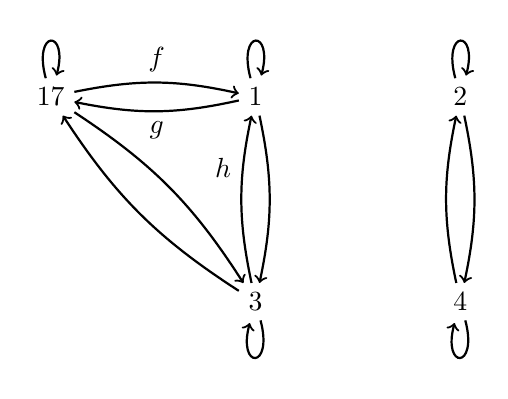
\begin{tikzpicture}[scale=1.3]
	\tikzset{arc lines/.style={thick,black, ->, bend left=12}}
	% \draw (0, 0) grid (6, 2);
	\node (17) at (0, 2) {$17$};
	\node (1) at (2, 2) {$1$};
	\node (2) at (4, 2) {$2$};
	\node (3) at (2, 0) {$3$};
	\node (4) at (4, 0) {$4$};
	\draw [arc lines] (17) to node[above] {$f$} (1);
	\draw [arc lines] (1) to node[below] {$g$} (17);
	\draw [arc lines] (17) to (3);
	\draw [arc lines] (3) to (17);
	\draw [arc lines] (1) to (3);
	\draw [arc lines] (3) to node[left, yshift=4mm] {$h$} (1);
	\draw [arc lines] (2) to (4);
	\draw [arc lines] (4) to (2);
	\path [-stealth, thick]
	(1) edge [loop above] (1)
	(17) edge [loop above] (17)
	(2) edge [loop above] (2)
	(3) edge [loop below] (3)
	(4) edge [loop below] (4)
	;
\end{tikzpicture}
\end{document}

	\end{center}
	\caption{Equivalence Relation}
\end{figure}
With this depiction, it's easy to see the cliques that create the
equivalence classes. Visually we can see that each object has an identity arrow,
and that the composition arrows have been omitted.

Let us check some of the objects and arrows for unitality and associativity.
\begin{align*}
	1_1 \circ f = & (1, 1) \circ (17, 1) &  &                  \\
	=             & (17, 1)                                    \\
	=             & f                    &  & \text{unitality} \\
	g \circ 1_1 = & (1, 17) \circ (1, 1)                       \\
	=             & (1, 17)                                    \\
	=             & g                    &  & \text{unitality} \\
\end{align*}
\begin{align*}
	(f \circ g) \circ h = & ((17, 1) \circ (1, 17)) \circ (3, 1)                           \\
	=                     & (1, 1) \circ (3, 1)                                            \\
	=                     & (3, 1)                                                         \\
	f \circ (g \circ h) = & (17, 1) \circ ((1, 17) \circ (3, 1))                           \\
	=                     & (17, 1) \circ (3, 17)                                          \\
	=                     & (3, 1)                               &  & \text{associativity} \\
\end{align*}
You get identities from reflexivity, inverses through symmetry, and composition
via transitivity.

\begin{ttta}
	\begin{enumerate}[label = {(\alph*)}]
		\item Check that equivalence relations create a category.
		\item What is the identity on each object and what is composition?
		\item Check that it satisfies the axioms.
		\item Conversely, can you put some conditions on a category to ensure that it is an equivalence relation?
	\end{enumerate}
\end{ttta}
\begin{proofitem}
	\item Let $S$ be a set and let $R\subseteq S\times S$ be an equivalence relation on $S$.
	\begin{align}
		x \in S \implies (x, x) \in R                  &  & \text{reflexivity}  \\
		(x,y) \in R \implies (y, x) \in R              &  & \text{symmetry}     \\
		(x,y) \land (y, z) \in R \implies (x, z) \in R &  & \text{transitivity}
	\end{align}
	\item
	Categories can be seen to be inspired by equivalence relations. Start with a set
	$S$ that has an equivalence relation $R$.
	\begin{enumerate}
		\item Objects: $x\in S$.
		\item Arrows: $a\in R\subseteq S\times S$.
	\end{enumerate}
	\item Let $\mathcal{C}_{\text{eq}}$ be the category formed from an equivalence
	relation.
	\item To show that $R$ and $S$ form a category, we must show that it adheres to
	the two required properties of categories: unitality and associativity.
	\item The unit laws requires that for any arrow $f:a \rightarrow b$, there
	exists arrows $1_a \land 1_b$ such $f\circ 1_a = f = 1_b \circ f$.
	\begin{figure}[H]
		\begin{align*}
			f=          & (a, b)            \\
			f\circ 1_a= & (a, b)\circ(a, a) \\
			=           & (a, b)            \\
			1_b\circ f= & (b, b)\circ(a, b) \\
			=           & (a, b)
		\end{align*}
		\caption{Unital Laws}
	\end{figure}
	\item Thus we have shown the category $\mathcal{C}_{\text{eq}}$ adheres to the unital laws.
	\begin{figure}[H]
		\begin{align*}
			f=                               & (a, b)                        \\
			g=                               & (b, c)                        \\
			h=                               & (c, d)                        \\
			\left((h\circ g)\circ f\right) = & ((c,d)\circ(b,c))\circ (a, b) \\
			=                                & (b,d)\circ (a, b)             \\
			=                                & (a, d)                        \\
			h\circ (g\circ f)=               & (c, d)\circ((b,c)\circ(a,b))  \\
			=                                & (c, d)\circ(a,c)              \\
			=                                & (a, d)
		\end{align*}
		\caption{Associative Laws}
	\end{figure}
	\item Thus we have shown the category $\mathcal{C}_{\text{eq}}$ adheres to the
	associative laws.

	\setcounter{tttacounter}{0}
	\begin{ttta}
		Conversely, can you put some conditions on a category to ensure that it
		“is” an equivalence relation?
	\end{ttta}
	\item To assure that some category $\mathcal{C}$ forms an equivalence relation,
	it must be shown that $\mathcal{C}$ gives rise to the three properties
	required for an equivalence relation: reflexivity, symmetry, and
	transitivity. Reflexivity and transitivity are guaranteed for any category
	via the unital and associative properties---requirements to be a category. To
	satisfy symmetry, for any arrow $f:a\rightarrow b\in \mathcal{C}_{\hom}$, there
	must exist an arrow $g:b\rightarrow a\in \mathcal{C}_{\hom}$.

	Additionally, there can be only arrow between any two objects $a, b \in
		\mathcal{C}_{ob}$. This uniqueness property between two objects is required
	because a relation $R$ is a set, and a set is defined by some characteristic
	function, which is a function with a boolean codomain. Either an element is
	in or out of the set, and more than one arrow between the same objects would
	violate this requirement.
\end{proofitem}

\begin{table}
	\centering % Optional, for centering the table
	\begin{tabular}{ ccccc } % 5 columns, each centered
		\toprule
		           & Equivalence Relation &               & Category      &            \\ \midrule
		Data       & objects              & $\rightarrow$ & objects       & Data       \\
		Structure  & relations            & $\rightarrow$ & arrows        &            \\ \midrule
		           & reflexivity          & $\rightarrow$ & identities    &            \\
		Properties & symmetry             & $\rightarrow$ & inverses      & Structure  \\
		           & transitivity         & $\rightarrow$ & composition   &            \\\midrule
		           &                      &               & unit laws     & Properties \\
		           &                      &               & associativity &
		\\\bottomrule
	\end{tabular}
	\caption{Equivalence Relation in set theory v.\;category theory}
\end{table}
\subsection{Factors as a Category}
Pick a number. The factors are the objects, and an arrow $a\rightarrow b$ exists
whenever $a$ is a factor of $b$. In this cateogry, like the equivalence-relation
category, there is at most one arrow between two objects. That is because this
category is a relation. Any relation $(a, b)$ can only be in
a set once, per the definition of set.
\begin{figure}[H]
	\begin{center}
		\documentclass[border=0.2cm]{standalone}
\usepackage{tikz}
\usepackage{titlesec}
\usepackage{float}
\usepackage{standalone}
\usepackage{tikzit}
\usetikzlibrary{automata, arrows.meta, positioning}
\usetikzlibrary{arrows.meta, positioning}
\input{sample-02.tikzstyles}

\begin{document}
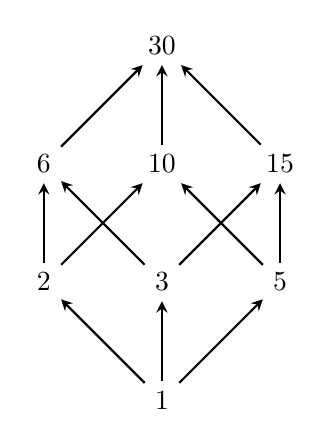
\begin{tikzpicture}[->, >=stealth, thick]
\node (1) at (3,0) {$1$};
\node (2) at (1.5,1.5) {$2$};
\node (3) at (3,1.5) {$3$};
\node (5) at (4.5,1.5) {$5$};
\node (6) at (1.5,3) {$6$};
\node (10) at (3,3) {$10$};
\node (15) at (4.5,3) {$15$};
\node (30) at (3,4.5) {$30$};
\draw (1) -- (2);
\draw (1) -- (3);
\draw (1) -- (5);
\draw (2) -- (6);
\draw (2) -- (10);
\draw (3) -- (6);
\draw (3) -- (15);
\draw (5) -- (10);
\draw (5) -- (15);
\draw (6) -- (30);
\draw (10) -- (30);
\draw (15) -- (30);
\end{tikzpicture}
\end{document}

	\end{center}
	\caption{30-factor Category}
\end{figure}
\stepcounter{tttacounter}
\begin{ttta}
	What would happen if we took our objects to be the whole of $\mathbb{N}$ instead?
\end{ttta}
If we took all of $\mathbb{N}$ as a category, then $0$ would be in
$\mathcal{C}_{ob}$, and there would need to be a identify morphism from $0$ to
itself. Because $0$ is a not a factor of any integer, there can't be an
identity arrow for $0$, so the natural numbers using a factor relationship for
morphisms would not form a category. If we modify the set to be $\mathbb{N} /
	\set{0}$, then there would be a morphism from $1$ to all other elements. $1$
the natural number is the initial object, paradoxically notated as the $0$
object. Each prime number would have two morphisms---the identity morphism and
one from $1$ to itself.
